\section{Funzioni lisce e reali analitiche}

\subsection{Funzioni lisce}

Consideriamo $ \R^{n} $ con $ n \geq 1 $ e $ U \subset \R^{n} $ aperto; prendiamo una funzione $ f : U \to \R $ e $ p \in U $: diremo che $ f \in C^{k} $in $ p $ con $ k \in \N $ se le derivate $ k $-esime di $ f $, definite come

\begin{equation}
	\pdv[k]{f}{x^{1} \cdots}{x^{k}} \qcomma k \in \N
\end{equation}

esistono e sono continue in $ p $.\\
Prendendo $ k = 0 $, abbiamo che

\begin{equation}
	f \in C^{0} \iff f \text{ continua}
\end{equation}

Diremo che:

\begin{itemize}
	\item $ f \in C^{k} $ in $ U $ se $ f \in C^{k} $ in $ p $ per $ \forall p \in U $
	
	\item $ f \in C^{\infty} $ o \textit{liscia} in $ p $ se $ f \in C^{k} $ in $ p $ per $ \forall k \in \N $
	
	\item $ f \in C^{\infty} $ o \textit{liscia} in $ U $ se $ f \in C^{\infty} $ per $ \forall p \in U $
\end{itemize}

perciò una funzione è liscia se esistono e sono finite le sue derivate di qualunque ordine.\\
Queste funzioni sono quelle su cui si basa il concetto di \textit{varietà differenziabile}.\\

Per generalizzare, consideriamo le funzioni definite non in $ \R $ ma in $ \R^{n} $.\\
Una funzione $ f : U \to \R^{n} $ con $ n \geq 1 $ e $ U \subset \R^{m} $ con $ m \geq 1 $ aperto è $ C^{k} $ in $ p $ se tutte le sue componenti $ f^{j} : U \to \R $ sono $ f^{j} \in C^{k} $ in $ p $ con $ k \geq 0 $. Nello specifico, $ f = (f^{1}, \dots, f^{m}) $ oppure $ f^{j} = \pi_{j} \circ f $ dove $ \pi_{j} $ è la proiezione $ \pi_{j} : \R^{m} \to \R $ con $ (x^{1}, \dots, x^{m}) \mapsto x^{j} $, $ j = 1, \dots, m $.\\
Una funzione $ f : U \to \R^{m} $ è:

\begin{itemize}
	\item $ C^{k} $ in $ U $ se $ f^{j} \in C^{k} $ in $ U $
	
	\item liscia in $ p \in U $ se $ f^{j} \in C^{\infty} $ in $ p $ per $ \forall j = 1, \dots, m $
	
	\item liscia in $ U $ se $ f^{j} \in C^{\infty} $ in $ U $ per $ \forall j = 1, \dots, m $
\end{itemize}

\subsubsection{\textit{Esempi}}

\paragraph{1.}

Sia

\map{f}
	{\R}{\R}
	{x}{x^{1/3}}
	
La funzione è continua ($ f \in C^{0} $) ed è un omeomorfismo\footnote{%
	Sia la funzione che la sua inversa sono continue.%
} ma $ f \notin C^{1} $ nell'origine $ p = 0 $ perché

\begin{equation}
	f^{\prime} = \dfrac{x^{-2/3}}{3}
\end{equation}

la quale non è definita nell'origine e dunque $ f \notin C^{1} (\R) $.

\paragraph{2.}

Se volessi costruire una funzione che sia $ C^{1} $ ma non $ C^{2} $, potrei integrare la $ f $ del punto precedente.\\
Sia $ g : \R \to \R $ con

\begin{equation}
	g (x) = \int_{0}^{x} f (t) \dd{t} = \dfrac{3 x^{2/3}}{4}
\end{equation}

da cui si ottiene che $ g \in C^{1} (\R) $ ma $ g \notin C^{2} (\R) $.

\paragraph{3.}

Vedi Esercizio \ref{es1-1}.

\subsection{Funzioni reali analitiche}

Dato $ p \in \R^{n} $, un intorno $ U $ di $ p $ è un aperto di $ \R^{n} $ che contiene $ p $.\\
Sia $ f : U \to \R $ con $ U \subset \R^{n} $ aperto, diremo che $ f $ è \textit{reale analitica} in $ p \in U $ se $ f $ coincide con il suo sviluppo di Taylor intorno a $ p $. Questo significa che se prendo una funzione $ f (x) $ con $ x = (x^{1}, \dots, x^{n}) $ e $ p = (p^{1}, \dots, p^{n}) $ ho che

\begin{align}
	\begin{split}
		f (x) &= f (p) + \sum_{i=1}^{n} \pdv{f}{x_{i}} (p) (x^{i} - p^{i}) + \cdots + \dfrac{1}{k!} \sum_{i_{1},\dots,i_{k}=1}^{n} \dfrac{\partial^{k} f}{\partial x^{i_{1}} \cdots \partial x^{i_{k}}} (p) ( (x^{i_{1}} - p^{i_{1}}) \cdots (x^{i_{k}} - p^{i_{k}}) ) + \cdots\\
		&= f (p) + \sum_{k=1}^{\infty} \dfrac{1}{k!} \sum_{i_{1},\dots,i_{k}=1}^{n} \dfrac{\partial^{k} f}{\partial x^{i_{1}} \cdots \partial x^{i_{k}}} (p) \prod_{j=1}^{k} (x^{j} - p^{j})
	\end{split}
\end{align}

Se abbiamo una serie di potenze, possiamo derivarla termine a termine dunque, siccome una funzione reale analitica coincide con il suo sviluppo in serie di Taylor, è possibile derivarla ottenendo sempre una funzione continua con derivata continua. A questo punto $ f \in C^{\infty} $: questo segue dall'analisi in quanto le serie di potenze possono essere derivate un numero arbitrario di volte.

\subsubsection{\textit{Esempi}}

\paragraph{1.}

La funzione $ f (x) = \sin x $ è liscia reale analitica e ha sviluppo di Taylor

\begin{align}
	\begin{split}
		\sin x &= x - \dfrac{x^{3}}{3!} + \dfrac{x^{5}}{5!} - \dots\\
		&= \sum_{j=0}^{\infty} (-1)^{j} \dfrac{x^{2j+1}}{(2j+1)!}
	\end{split}
\end{align}

Per calcolare la derivata possiamo derivare termine a termine lo sviluppo di Taylor

\begin{align}
	\begin{split}
		\dv{x} \sin x &= \dv{x} \sum_{j=0}^{\infty} (-1)^{j} \dfrac{x^{2j+1}}{(2j+1)!}\\
		&= \sum_{j=0}^{\infty} (-1)^{j} (2j+1) \dfrac{x^{2j}}{(2j+1)!}\\
		&= \sum_{j=0}^{\infty} (-1)^{j} \dfrac{x^{2j}}{(2j)!}\\
		&= \cos x
	\end{split}
\end{align}

\paragraph{2.}

Per trovare la derivata di $ f(x) = e^{x} $ ripetiamo lo stesso procedimento

\begin{align}
	\begin{split}
		\dv{x} e^{x} &= \dv{x} \sum_{j=0}^{\infty}\dfrac{x^{j}}{j!}\\
		&= \sum_{j=0}^{\infty} j \, \dfrac{x^{j-1}}{j!}\\
		&= \sum_{j=0}^{\infty} \dfrac{x^{j-1}}{(j-1)!}\\
		&= \sum_{n=-1}^{\infty} \dfrac{x^{n}}{n!}\\
		&= \sum_{n=0}^{\infty} \dfrac{x^{n}}{n!}\\
		&= e^{x}
	\end{split}
\end{align}

\paragraph{3.}

Un esempio di funzione liscia ma non reale analitica è

\map{f}
	{\R}{\R}
	{x}{%
		\begin{cases}
			e^{-1/x^{2}},& \text{se } x > 0\\
			0,& \text{se } x \leqslant 0
		\end{cases}
		}

Per controllare che sia $ C^{0} $ dobbiamo verificare che

\begin{equation}
	\lim_{x \to 0} e^{-1/x^{2}} = 0
\end{equation}

Per controllare che sia liscia

\begin{equation}
	\lim_{x \to 0} f^{\prime} (x) = \lim_{x \to 0} \left(\dfrac{2}{x^{3}}\right) e^{-1/x^{2}} = 0
\end{equation}

Vedi Esercizio \ref{es1-2}.

Tutto questo ci dice che $ f \in C^{\infty}(\R) $. Se fosse anche reale analitica, dovrebbe coincidere con il suo sviluppo in serie di Taylor anche nell'origine, dunque

\begin{align}
	\begin{split}
		f(x) = \sum_{k=0}^{\infty} \pdv[k]{f}{x} (0) \, x^{k}
	\end{split}
\end{align}

ma $ f(x) $ nell'intorno di 0 è nulla solo per $ x \leqslant 0 $ mentre lo sviluppo di Taylor è sempre nullo: questa contraddizione porta a dire che, nonostante $ f \in C^{\infty}(\R) $, questa non è reale analitica, scritto anche come $ f \notin C^{\omega}(\R) $.\\
Un altro motivo per il quale $ f \notin C^{\omega}(\R) $ segue dal fatto che se $ f : U \to \R $ con $ U \in \R $ aperto è reale analitica e $ f = 0 $ in un aperto, allora $ f \equiv 0 $ ovunque\footnote{%
	Vale anche se è uguale per una costante diversa da 0.}.

\section{Diffeomorfismi tra aperti di $ \R^{n} $}

Prendiamo $ U, V \in \R^{n} $ aperti, diremo che $ f : U \to V $ è un \textit{diffeomorfismo} se è una bigezione\footnote{%
	Perciò è invertibile.%
}, $ f \in C^{\infty} $ e la sua inversa $ g : V \to U $ è  $ g \in C^{\infty} $.\\
Ad esempio, la funzione

\map{f}
	{\R}{\R}
	{x}{x^{3}}
	
è una bigezione, è liscia ma la sua inversa non lo è, dunque $ f $ non è un diffeomorfismo.\\
Quando esiste un diffeomorfismo tra due aperti, si dice che questi sono \textit{diffeomorfi}: $ U $ e $ V $ sono diffeomorfi se $ \E f : U \to V $ diffeomorfismo, i.e. $ U \simeq V $.\\

\begin{theorem}[Invarianza topologica della dimensione]
	Se $ U \subset \R^{n} $ e $ V \subset \R^{m} $ sono aperti omeomorfi allora $ n = m $.
\end{theorem}

\begin{theorem}[Invarianza differenziabile della dimensione]
	Se $ U \subset \R^{n} $ e $ V \subset \R^{m} $ sono aperti diffeomorfi allora $ n = m $\footnote{%
		Questo teorema implica quello di "Invarianza topologia della dimensione" in quanto la condizione di diffeomorfismo implica quella di omeomorfismo.}.
\end{theorem}

È naturale verificare se gli spazi legati da omeomorfismi siano legati anche da diffeomorfismi.\\
I seguenti sottoinsiemi aperti di $ \R $:

\begin{itemize}
	\item $ (a,b) $ con $ a < b $
	
	\item $ \R $
	
	\item $ (c, + \infty) $
	
	\item $ (- \infty, d) $
\end{itemize}

sono diffeomorfi tra loro\footnote{%
	Vedi Esercizio \ref{es1-3}.%
} per $ \forall a,b,c,d \in \R $.

\subsection{Diffeomorfismo tra $ B_{\delta} (c) $ e $ \R^{n} $}

Indichiamo con $ B_{1} (0) $ la \textit{palla} di centro l'origine e raggio unitario, i.e.

\begin{equation}
	B_{1} (0) = \left\{ x \in \R^{n} \st \norm{x} \doteq \sqrt{\sum_{i=1}^{n} (x^{i})^{2}} < 1 \right\}
\end{equation}

Per $ n=1 $, $ B_{1} (0) \equiv (-1,1) \simeq \R $.\\
Definiamo

\map{f}
	{B_{1} (0)}{\R^{n}}
	{x}{\left( \dfrac{x^{1}}{\sqrt{1 - \norm{x}^{2}}}, \cdots, \dfrac{x^{n}}{\sqrt{1 - \norm{x}^{2}}} \right)}

questa applicazione è un diffeomorfismo. Per verificarlo, dobbiamo dimostrare che $ f $ sia un bigezione, $ f \in C^{\infty} $ e che $ f^{-1} \in C^{\infty} $.\\
L'inversa è

\map{f}
	{\R^{n}}{B_{1} (0)}
	{x}{\left( \dfrac{x^{1}}{\sqrt{1 + \norm{x}^{2}}}, \cdots, \dfrac{x^{n}}{\sqrt{1 + \norm{x}^{2}}} \right)}

in quanto

\begin{equation}
	f \circ g = \id_{\R^{n}} \wedge g \circ f = \id_{B_{1} (0)}
\end{equation}

Perché sia $ f $ che $ f^{-1} $ siano lisce, dobbiamo verificare che ogni loro componente lo sia, il quale è verificato perché la derivata di una delle componenti di $ f $ ha al denominatore sempre $ \sqrt{1 - \norm{x}^{2}} \in B_{1} (0) $ e lo stesso vale per la sua inversa $ \sqrt{1 + \norm{x}^{2}} \in \R^{n} $.

\begin{corollary}
	La palla di centro $ c $ e raggio $ \delta $ con $ c \in \R^{n} $ e $ \delta \geqslant 0 $ è diffeomorfa a $ \R^{n} $, i.e. $ B_{\delta} (c) \simeq \R^{n} $.
\end{corollary}

Per dimostrare questo è necessario dimostrare che siano diffeomorfismi le traslazioni (le quali sono lineari e affini) e le omotetie (scala di un fattore $ \delta $); questa dimostrazione mostra anche che $ B_{1} (0) \simeq B_{\delta} (c) $.\\
Vedi Esercizio \ref{es1-4}.\\
Per praticità di notazione, chiamiamo $ h $ il diffeomorfismo $ B_{\delta} (c) \to \R^{n} $ definito sopra. Per far vedere come nasce questo diffeomorfismo, si può usare la seguente costruzione geometrica

\begin{figure}[H]
	\centering

	\begin{tikzpicture}[scale=1]
	
		\begin{axis}[
					axis lines=center,
					anchor=origin,
					axis equal=true,
					xlabel={$ (x^{1}, \dots, x^{n}) $},
					ylabel=$ x^{n+1} $,
					xticklabel=\empty,
					yticklabel=\empty,
					xlabel style = {anchor=south west},
					ylabel style = {anchor=south},
					xmax=2.5,
					xmin=-1.5,
					ymax=1.5,
					ymin=-0.5
					]
			
			\addplot[
					samples=1000, 
					color=black,
					]
			{1-sqrt(1-x^2)};
			
			\addplot[
					domain=0:2,
					samples=1000, 
					color=red,
					]
			{1-x/2};
			
			\addplot[
					samples=1000, 
					color=black,
					dashed,
					]
			coordinates {(1,0)(1,1)};
			
			\addplot[
					samples=1000, 
					color=black,
					dashed,
					]
			coordinates {(-1,0)(-1,1)};
			
			\addplot[
					color=red,
					mark=*,
					]
			coordinates {(0,1)};
			
			\addplot[
					color=red,
					mark=*,
					]
			coordinates {(2,0)};
			
			\addplot[
					color=blue,
					mark=*,
					]
			coordinates {(0,1)};
			
			\addplot[
					color=blue,
					mark=*,
					]
			coordinates {(2,0)};

		\end{axis}
	
	\end{tikzpicture}

\end{figure}

Consideriamo la semicalotta aperta in $ \R^{n+1} $ centrata in $ (0,\dots,0,1) $ di raggio $ 1 $:

\begin{equation}
	S = \left\{ (x^{1}, \dots, x^{n+1}) \in \R^{n+1} \st (x^{n+1})^{2} + \sum_{i=1}^{n} (x^{i})^{2} = 1 \, \wedge \, x^{n+1} < 1 \right\}
\end{equation}

La palla $ B_{1}(0) $ vive nella proiezione della semicalotta sull'iperpiano $ (x^{1}, \dots, x^{n}) $, definita come

\begin{equation}
	B_{1}(0) = \left\{ x \in \R^{n} \st \norm{x} < 1 \right\}
\end{equation}

Questa proiezione permette di costruire l'applicazione $ h $ in due passaggi: prima prendiamo un punto in $ B_{1}(0) $, lo proiettiamo su $ S $ e, con una proiezione stereografica, lo portiamo su $ \R^{n} $. La prima applicazione è $ f : B_{1}(0) \to S $ mentre la seconda $ g : S \to \R^{n} $, cioè la proiezione stereografica dal punto $ (0,\dots,0,1) $. Abbiamo dunque che $ g \circ f = h $. Le mappe sono

\begin{equation}
	f (x^{1},\dots,x^{n+1}) = \left( x^{1},\dots,x^{n},1-\sqrt{1-\norm{x}^{2}} \right)
\end{equation}

\begin{equation}
	g (x^{1},\dots,x^{n+1}) = \left( \dfrac{x^{1}}{1-x^{n+1}},\dots,\dfrac{x^{n}}{1-x^{n+1}},0 \right)
\end{equation}

da cui

\begin{align}
	\begin{split}
		h (x^{1},\dots,x^{n+1}) &= (g \circ f) (x^{1},\dots,x^{n+1})\\
		&= g \left( x^{1},\dots,x^{n},1-\sqrt{1-\norm{x}^{2}} \right)\\
		&= \left( \dfrac{x^{1}}{\sqrt{1 - \norm{x}^{2}}}, \cdots, \dfrac{x^{n}}{\sqrt{1 - \norm{x}^{2}}}, 0 \right)
	\end{split}
\end{align}

A questo punto $ B_{1} (0) \simeq \R^{n} $: dal punto di vista della geometria differenziale, due oggetti diffeomorfi vengono considerati equivalenti\footnote{%
	In topologia, vale lo stesso ragionamento per oggetti omeomorfi.}.

\subsection{Teorema di Taylor con resto}

Una funzione reale analitica coincide con il suo sviluppo di Taylor. Per una funzione liscia questo non è detto: la coincidenza di una funzione liscia con il suo sviluppo di Taylor è data a meno di un \textit{resto}. Introduciamo ora il concetto di insieme stellato rispetto a un punto per definire il resto sopraccitato.\\
Un sottoinsieme aperto $ U \subset \R^{n} $ è \textit{stellato} rispetto a un punto $ p \in U $ se il segmento di retta che unisce $ p $ a $ \forall x \in U $ è interamente contenuto in $ U $.

\begin{remark}
	Un insieme convesso è stellato rispetto a ogni suo punto.
\end{remark}

L'ipotesi che un sottoinsieme sia stellato è forte a livello globale ma sempre rispettata a livello locale, in quanto è sempre possibile trovare un aperto stellato rispetto a un punto all'interno di un insieme.

\begin{theorem}[Taylor con resto]
	Sia $ f : U \to \R $ con $ U \subset \R^{n} $ stellato rispetto a un punto $ p \in U $ e supponiamo $ f \in C^{\infty}(U) $, allora esistono $ n $ funzioni $ g_{i} \in C^{\infty}(U) $ per $ i = 1,\dots,n $ definite come
	
	\begin{equation}
		g_{i}(p) \doteq \pdv{f}{x^{i}} \, (p) \qcomma \forall i=1,\dots,n
	\end{equation}

	tali che
	
	\begin{equation}
		f(x) = f(p) + \sum_{i=1}^{n} (x^{i}-p^{i}) \, g_{i}(x) \qcomma \forall x \in U
	\end{equation}	
\end{theorem}

\begin{proof}
	Consideriamo il segmento $ r $ che  unisce $ p $ a un punto $ x \in U $ con $ x $ fissato  arbitrariamente:
	
	\begin{equation}
		r=p+t(x-p) \qcomma t \in [0,1]
	\end{equation}
	
	Essendo $ U $ stellato rispetto a $ p $, possiamo valutare $ f $ in questo segmento (tutti i punti di $ r $ sono definiti in $ U $). Considero fissi $ x $ e $ p $ e derivo $ f(r) $ rispetto a $ t $
	
	\begin{align}
		\begin{split}
			\dv{t} f(r) &= \dv{t} f(p+t(x-p))\\
			&= \sum_{i=1}^{n} \pdv{f}{x^{i}} \, (p+t(x-p)) \, \left( \dv{r}{t} \right)^{i}\\
			&= \sum_{i=1}^{n} \pdv{f}{x^{i}} \, (p+t(x-p)) \, (x^{i}-p^{i})
		\end{split}
	\end{align}
	
	per la \textit{regola della catena}.\\
	Integrando rispetto a $ t $ nell'intervallo $ [0,1] $ ottengo
	
	\begin{align}
		\begin{split}
			\int_{0}^{1} \dv{t} f(p+t(x-p)) \dd{t} &= \int_{0}^{1} \sum_{i=1}^{n} \pdv{f}{x^{i}} \, (p+t(x-p)) \, (x^{i}-p^{i}) \dd{t}\\
			f(x) - f(p)&= \sum_{i=1}^{n} (x^{i}-p^{i}) \int_{0}^{1} \pdv{f}{x^{i}} \, (p+t(x-p)) \dd{t}
		\end{split}
	\end{align}
	
	chiamando
	
	\begin{equation}
		g_{i}(x) \doteq \int_{0}^{1} \pdv{f}{x^{i}} \, (p+t(x-p)) \dd{t}
	\end{equation}
	
	si può scrivere
	
	\begin{equation}
		f(x)= f(p) + \sum_{i=1}^{n} (x^{i}-p^{i}) \, g_{i}(x)
	\end{equation}
	
	dove $ g_{i}(x) \in C^{\infty}(U) $ perché derivata parziale di una funzione liscia.\\
	Inoltre
	
	\begin{equation}
		g_{i}(p) = \int_{0}^{1} \pdv{f}{x^{i}} \, (p) \dd{t} = \pdv{f}{x^{i}} \, (p) \qcomma \forall i=1,\dots,n
	\end{equation}
\end{proof}

Prendiamo $ f : U \to \R $ con $ p $ corrispondente all'origine. Per il teorema di Taylor con resto, sappiamo che esiste una funzione $ g_{1} \in C^{\infty}(U) $ tale che $ f(x) = f(0) + x \, g_{1}(x) $ con $ g_{1}(0) = f^{\prime}(0) $. Riapplicando il teorema a $ g_{1} $ (siccome è liscia), si ottiene che $ g_{1}(x) = g_{1}(0) + x g_{2}(x) $ con $ g_{2} \in C^{\infty}(U) $ e $ g_{2}(0) = g_{1}^{\prime}(0) $. Per induzione $ g_{i}(x) = g_{i}(0) + x g_{i+1}(x) $ dove $ g_{i+1} \in C^{\infty} (U) $ e $ g_{i+1}(0) = g_{i}^{\prime}(0) $ per $ \forall i \geqslant 1 $. Sostituendo in $ f $ tutte queste funzioni, si ottiene

\begin{align}
	\begin{split}
			f(x) &= f(0) + x g_{1}(x)\\
			&= f(0) + x g_{1}(0) + x^{2} g_{2}(x)\\
			&= f(0) + x g_{1}(0) + x^{2} g_{2}(0) + x^{3} g_{3}(x)\\
			& \;\, \vdots\\
			&= f(0) + x g_{1}(0) + \dots + x^{k} g_{k}(0) + x^{k+1} g_{k+1}(x)
	\end{split}
\end{align}

A questo punto si può identificare

\begin{equation}
	g_{k}(0) = \dfrac{1}{k!} \pdv[k]{f}{x} \, (0) \doteq \dfrac{f^{(k)}(0)}{k!}
\end{equation}

da cui

\begin{equation}
	f(x) = f(0) + \sum_{k=1}^{i} \dfrac{x^{k}}{k!} f^{(k)} (0) + x^{i+1} g_{i+1}(x) \qcomma \forall i \in \N
\end{equation}

dove la prima parte coincide con lo sviluppo in serie di Taylor mentre l'ultimo termine indica il \textit{resto}.\\
Vedi Esercizi \ref{es1-5} e \ref{es1-6}.

\section{Vettori tangenti in $ \R^{n} $}

Preso un punto $ p \in \R^{n} $, lo \textit{spazio tangente} in quel punto viene scritto $ T_{p}(\R^{n}) $. Lo spazio tangente a un punto $ p $ è l'insieme\footnote{%
	Formalmente, è uno spazio vettoriale con origine il punto $ p $.%
} di tutti i vettori che escono dal punto stesso. Essendo $ T_{p}(\R^{n}) \simeq \R^{n} $, un elemento $ v \in T_{p}(\R^{n}) $ è dunque un \textit{vettore riga o colonna}

\begin{equation}
	\bmqty{ v^{1} \\ \vdots \\ v^{n} } \qquad \lor \qquad \bmqty{ v^{1} & \cdots & v^{n} }
\end{equation}

dove le $ v^{i} $ sono le componenti del vettore nella base canonica, i.e.

\begin{equation}
	v = \sum_{i=1}^{n} v^{i} e_{i}
\end{equation}

Per generalizzare questo concetto, consideriamo gli elementi degli spazi tangenti non più come oggetti geometrici vettori ma come \textit{derivazioni}.

\subsection{Derivate direzionali}

Siano $ f : U \to \R $ con $ f \in C^{\infty}(\R^{n}) $, $ p\in U \subset \R^{n} $ e $ v \in T_{p}(\R^{n}) $. Consideriamo la retta $ c(t) $ che passa per $ p $ con direzione $ v $, parametrizzata come

\begin{equation}
	c(t) = p + t v \qcomma t \in \R
\end{equation}

Definiamo la \textit{derivata direzionale} di $ f $ rispetto a $ v $ come

\begin{align}
	\begin{split}
		D_{v} f \doteq& \, \lim_{t \to 0} \dfrac{f(c(t)) - f(p)}{t}\\
		&= \left. \dv{t} f(c(t)) \right|_{t=0}\\
		&= \sum_{i=1}^{n} \pdv{f}{x^{i}} \, (p) \left( \dv{t} c(t) \right)^{i}\\
		&= \sum_{i=1}^{n} \pdv{f}{x^{i}} \, (p) \, v^{i}
	\end{split}
\end{align}

dove $ D_{v} f \in \R $ e $ v = [v^{1},\dots,v^{n}] $.

\begin{remark}
	Sia $ g \in C^{\infty} (\R^{n}) $ tale che $ g : V \to \R $ con $ V \subset \R $ e $ V \cap U \neq \emptyset $. Se $ g \equiv f $ in un intorno del punto $ p \in U \cap V $, allora la loro derivata direzionale è la stessa\footnote{%
		Questo perché il limite del rapporto incrementale nella definizione di $ D_{v} f $ dipende da un intorno arbitrariamente piccolo.%
	}, i.e. $ D_{v} g = D_{v} f $.
\end{remark}

\begin{figure}[H]
	\centering
	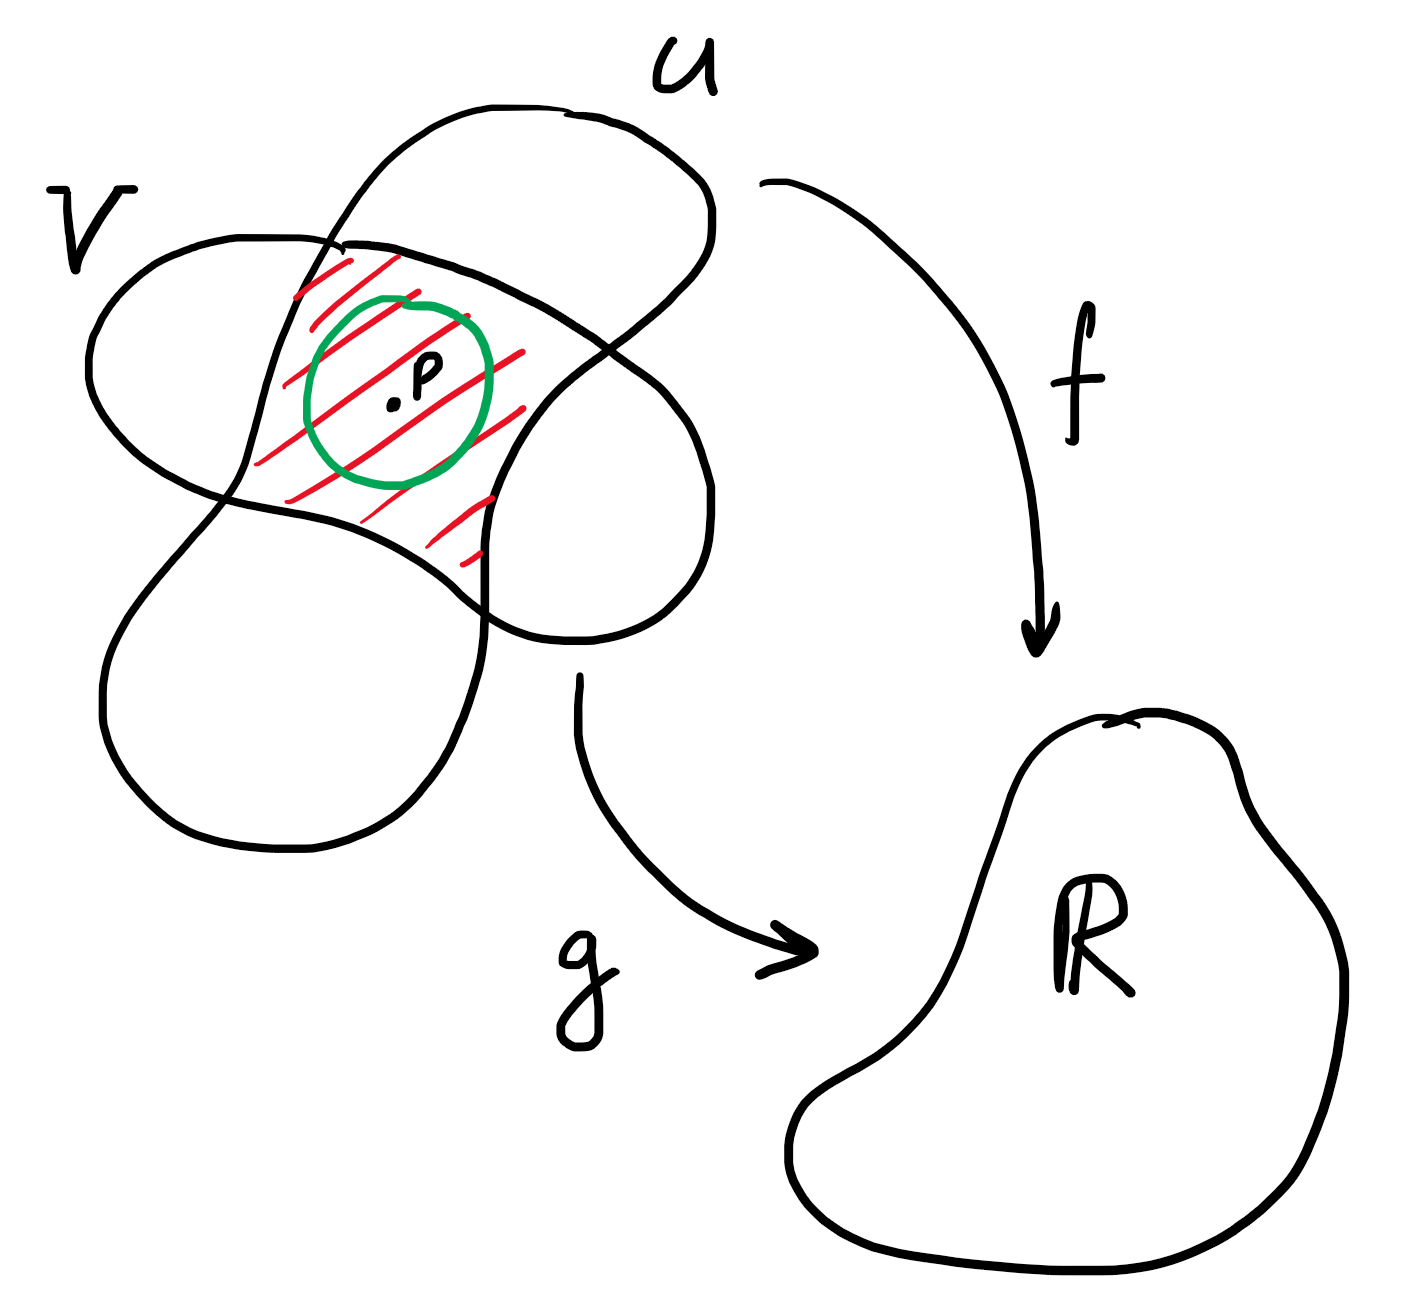
\includegraphics[width=0.4\textwidth,keepaspectratio]{img1}
\end{figure}

Definiamo ora l'insieme di coppie

\begin{equation}
	X \doteq \left\{ (f,U) \st f \in C^{\infty}(U), \, U \text{ intorno di } p \in U \right\}
\end{equation}

Diremo che\footnote{%
	Il simbolo $ \sim $ indica una relazione di equivalenza.%
} per $ p \in W $

\begin{equation}
	(f,U) \sim (g,V) \iff \E W \subseteq U \cap V, \, W \ni p \mid f(q) = g(q) \qcomma \forall q \in W
\end{equation}

Questa è effettivamente una relazione di equivalenza in quanto riflessiva, simmetrica e transitiva.\\
Prendiamo dunque lo spazio quoziente

\begin{equation}
	\sfrac{X}{\sim} \doteq C_{p}^{\infty}(\R^{n})
\end{equation}

dove un elemento $ [(f,U)] $ di questo spazio è chiamato \textit{germe} intorno al punto $ p $ ed è una \textit{classe di equivalenza} di coppie $ (f,U) $. A questo punto, $ C_{p}^{\infty}(\R^{n}) $ è l'insieme dei germi di funzioni lisce intorno a $ p $, i.e.

\begin{equation}
	C_{p}^{\infty}(\R^{n}) = \left\{ [(f,U)] \right\}
\end{equation} 

Possiamo definire un'applicazione

\map{D_{v}}%
	{C_{p}^{\infty}(\R^{n})}{\R}%
	{[(f,U)]}{D_{v} f}

Questa applicazione è ben definita in quanto l'associazione di un germe di funzioni a un numero reale non dipende dal rappresentante scelto perché

\begin{equation}
	(f,U) \sim (g,V) \implies D_{v} g = D_{v} f
\end{equation}

\subsubsection{\textit{Esempio}}

Siano $ f $ e $ g $

\begin{equation}
	\begin{cases}
		f(x) = \dfrac{1}{1-x}, & x \in \R \setminus \{1\}\\\\
		g(x) = \displaystyle\sum_{j=1}^{+\infty} x^{j}, & x \in (-1,1)
	\end{cases}
\end{equation}

Nonostante $ f\neq g $, nell'intorno $ (-1,1) $ di $ p=0 $ vale l'equivalenza per i germi

\begin{equation}
	(f,\R \setminus \{1\}) \sim (g,(-1,1))
\end{equation}

in altre parole, le classi di equivalenza

\begin{equation}
	[(f,\R \setminus \{1\})] = [(g,(-1,1))] \in C_{0}^{\infty}(\R)
\end{equation}

\subsubsection{Algebra su campo $ \K $}

Un'algebra $ A $ su un campo $ \K $ è una coppia $ (V,\cdot) $ con $ V $ spazio vettoriale su un campo $ \K $\footnote{%
	Dunque con operazioni
	\begin{equation}
		\begin{cases}
			a+b \in A, & \forall a,b \in A\\
			\lambda a \in A, & \forall \lambda \in \K
		\end{cases}
	\end{equation}%
} e un'operazione binaria

\map{\cdot}%
	{A \times A}{A}%
	{(a,b)}{a \cdot b}

tale che soddisfi le condizioni

\begin{equation}
	\begin{cases}
		(a \cdot b) \cdot c = a \cdot (b \cdot c) & \text{associatività}\footnotemark\\
		\begin{split}
			(a + b) \cdot c = a \cdot c + b \cdot c\\
			c \cdot (a + b) = c \cdot a + c \cdot b
		\end{split} & \text{distributività}\\
	\lambda (a \cdot b) = (\lambda a) \cdot b = a \cdot (\lambda b) & \text{omogeneità}
	\end{cases}
\footnotetext{In generale, non è necessaria l'associatività per definire un'algebra.}
\end{equation}

per $ \forall a,b,c \in A $ e $ \forall \lambda \in \K $.\\
Equivalentemente, un algebra su un campo $ \K $ può essere pensata come un anello\footnote{%
	Le proprietà di associatività e distributività sono sufficienti per renderla un anello.%
} $ (V,+,\cdot) $ il quale sia anche uno spazio vettoriale con aggiunta la proprietà di omogeneità.

\subsection{$ C_{p}^{\infty}(\R^{n}) $ come algebra su $ \R $}

Definiamo la somma

\begin{equation}
	[(f,U)] + [(g,V)] = [(f + g,U \cap V)] \qcomma [(f,U)], [(g,V)] \in C_{p}^{\infty}(\R^{n})
\end{equation}

Questa somma è ben definita in quanto, prendendo due rappresentanti qualsiasi di $ [(f,U)] $ e $ [(g,V)] $, esiste sempre un intorno in cui questa somma sia definita.\\
Allo stesso modo, definiamo il prodotto

\begin{equation}
	[(f,U)] \cdot [(g,V)] = [(f g,U \cap V)] \qcomma [(f,U)], [(g,V)] \in C_{p}^{\infty}(\R^{n})
\end{equation}

e la moltiplicazione per scalari

\begin{equation}
	\lambda [(f,U)] = [(\lambda f,U)] \qcomma \lambda \in \R
\end{equation}

Tutte queste operazioni sono ben definite e soddisfano tutte le proprietà di un'algebra perché la somma, il prodotto e la moltiplicazione per uno scalare di funzioni liscia soddisfano queste stesse proprietà.\\
A questo punto si può dire che $ C_{p}^{\infty}(\R^{n}) $ sia un'algebra su $ \R $.\\
Nonostante non sia necessario per un'algebra, $ C_{p}^{\infty}(\R^{n}) $ è anche commutativa e unitaria\footnote{%
	Vedi Esercizio \ref{es1-7}.%
} su $ \R^{n} $.

\subsection{Derivazione puntuale di $ C_{p}^{\infty}(\R^{n}) $}

A questo punto, possiamo definire l'applicazione chiamata \textit{derivazione puntuale} dell'algebra $ C_{p}^{\infty}(\R^{n}) $:

\map{D}%
	{C_{p}^{\infty}(\R^{n})}{\R}%
	{[(f,U)]}{D_{v} f = \sum_{i=1}^{n} \pdv{f}{x^{i}} \, (p) \, v^{i}}

con $ p \in U \subset \R^{n} $ e $ v = [v^{1}, \dots, v^{n}] \in T_{p} (\R^{n}) $.\\
Questa applicazione possiede le seguenti proprietà:

\begin{enumerate}
	\item $ \R $-linearità\footnote{%
		Rispetto alla struttura di spazio vettoriale di $ C_{p}^{\infty}(\R^{n}) $.%
	}, i.e.
		\begin{align}
			\begin{split}
				D ([(f,U)] + [(g,V)]) &= D ([(f,U)]) + D ([(g,V)])\\
				D (\lambda [(f,U)]) &= \lambda D ([(f,U)])
			\end{split}
		\end{align}
	
	\item soddisfa la \textit{regola di Leibniz}, i.e.
		\begin{equation}
			D ([(f,U)] \cdot [(g,V)]) = D ([(f,U)]) \, g(p) + f(p) \, D ([(g,V)])
		\end{equation}
\end{enumerate}

\begin{proof}[Dimostrazione ($ \R $-linearità (somma))]
	\begin{align}
		\begin{split}
			D ([(f,U)] + [(g,V)]) &= D ([(f+g,U \cap V)])\\
			&= D_{v} (f+g)\\
			&= \sum_{j=1}^{n} \pdv{(f+g)}{x^{j}} \, (p) \, v^{j}\\
			&= \sum_{j=1}^{n} \pdv{f}{x^{j}} \, (p) \, v^{j} + \sum_{j=1}^{n} \pdv{g}{x^{j}} \, (p) \, v^{j}\\
			&= D_{v} f + D_{v} g\\
			&= D ([(f,U)]) + D ([(g,V)])
		\end{split}
	\end{align}

	per $ \forall [(f,U)], [(g,V)] \in C_{p}^{\infty}(\R^{n}) $, $ \forall p \in U \cap V \subset \R^{n} $ e $ \forall v \in T_{p} (\R^{n}) $.
\end{proof}

\begin{proof}[Dimostrazione ($ \R $-linearità (moltiplicazione per scalare))]
	\begin{align}
		\begin{split}
			D (\lambda [(f,U)]) &= D ([(\lambda f,U)])\\
			&= D_{v} (\lambda f)\\
			&= \sum_{j=1}^{n} \pdv{(\lambda f)}{x^{j}} \, (p) \, v^{j}\\
			&= \lambda \sum_{j=1}^{n} \pdv{f}{x^{j}} \, (p) \, v^{j}\\
			&= \lambda D ([(f,U)])
		\end{split}
	\end{align}

	per $ \forall [(f,U)], [(g,V)] \in C_{p}^{\infty}(\R^{n}) $, $ \forall \lambda \in \R $, $ \forall p \in U \subset \R^{n} $ e $ \forall v \in T_{p} (\R^{n}) $.
\end{proof}

\begin{proof}[Dimostrazione (Regola di Leibniz)]
	\begin{align}
		\begin{split}
			D ([(f,U)] \cdot [(g,V)]) &= D ([(f g,U \cap V)])\\
			&= D_{v} (f g)\\
			&= \sum_{j=1}^{n} \pdv{(f g)}{x^{j}} \, (p) \, v^{j}\\
			&= \left( \sum_{j=1}^{n} \pdv{f}{x^{j}} \, (p) \, v^{j} \right) \, g(p) + f(p) \left( \, \sum_{j=1}^{n} \pdv{g}{x^{j}} \, (p) \, v^{j} \right)\\
			&= (D_{v} f) \, g(p) + f(p) \, (D_{v} g)\\
			&= D ([(f,U)]) \, g(p) + f(p) \, D ([(g,V)])
		\end{split}
	\end{align}

	per $ \forall [(f,U)], [(g,V)] \in C_{p}^{\infty}(\R^{n}) $, $ \forall p \in U \cap V \subset \R^{n} $ e $ \forall v \in T_{p} (\R^{n}) $.
\end{proof}

La derivazione puntuale è quindi un modo per associare un numero reale a un germe di funzioni, soddisfacendo le proprietà definite sopra.\\
Indichiamo dunque l'insieme delle derivazioni puntuali di $ C_{p}^{\infty}(\R^{n}) $ come $ \der_{p}(C_{p}^{\infty}(\R^{n})) $, i.e.

\begin{equation}
	\der_{p}(C_{p}^{\infty}(\R^{n})) \doteq \left\{ D ([(f,U)]) = D_{v} f \doteq \sum_{j=1}^{n} \pdv{f}{x^{j}} \, (p) \, v^{j} \in \R \st [(f,U)] \in C_{p}^{\infty}(\R^{n}), v \in T_{p} (\R^{n}) \right\}
\end{equation}

\subsection{Isomorfismo tra $ T_{p}(\R^{n}) $ e $ \der_{p}(C_{p}^{\infty}(\R^{n})) $}

Definiamo l'applicazione

\begin{align}
	\begin{split}
		\phi : T_{p}(\R^{n}) &\to \der_{p}(C_{p}^{\infty}(\R^{n}))\\
		v &\mapsto D_{v}
	\end{split}
\end{align}

questa associa il vettore $ v = [v^{1},\dots,v^{n}] \in T_{p}(\R^{n}) $ con $ p \in \R^{n} $ alla derivazione puntuale $ D_{v} $, la quale è a sua volta un'applicazione che associa la classe di equivalenza di germi di funzioni $ [(f,U)] $ alla derivata direzionale di $ f $ rispetto a $ v $, i.e.

\begin{align}
	D_{v} f = \sum_{j=1}^{n} \dfrac{\partial f}{\partial x^{j}} (p) \, v^{j} \in \R
\end{align}

Possiamo usare lo stesso simbolo, i.e. $ D_{v} ([(f,U)]) = D_{v} f $, perché questa relazione vale per qualsiasi rappresentante della classe.\\
L'applicazione $ \phi $ permette di considerare equivalentemente l'insieme delle derivazioni puntuali dell'algebra dei germi delle funzioni $ C_{p}^{\infty}(\R^{n}) $ e lo spazio tangente a un punto, in quanto questi due insiemi sono isomorfi tra loro tramite $ \phi $ stessa. Utilizzare le derivazioni è utile perché per le varietà differenziabili non esiste una visualizzazione dello spazio tangente.

\begin{theorem}
	L'applicazione $ \phi $ è un isomorfismo degli spazi vettoriali $ T_{p}(\R^{n}) $ e $ \der_{p}(C_{p}^{\infty}(\R^{n})) $, i.e. tramite $ \phi $ si ha che
	
	\begin{equation}
		T_{p}(\R^{n}) \stackrel{iso.}{\simeq} \der_{p}(C_{p}^{\infty}(\R^{n}))
	\end{equation}
\end{theorem}

Per dimostrare questo teorema è necessario notare che gli elementi $ D_{i} \in \der_{p}(C_{p}^{\infty}(\R^{n})) $ costituiscono uno spazio vettoriale\footnote{%
	Vedi Esercizio \ref{es1-8}.%
} con operazioni

\map{+}
	{\der_{p}(C_{p}^{\infty}(\R^{n})) \times \der_{p}(C_{p}^{\infty}(\R^{n}))}{\der_{p}(C_{p}^{\infty}(\R^{n}))}
	{(D_{v}, D_{w})}{D_{v} + D_{w}}
	
\map{\cdot}
	{\R \times \der_{p}(C_{p}^{\infty}(\R^{n}))}{\der_{p}(C_{p}^{\infty}(\R^{n}))}
	{(\lambda, D_{v})}{\lambda D_{v}}

Consideriamo ora la seguente preposizione:

\begin{definition}
	Le operazioni dello spazio vettoriale $ \der_{p}(C_{p}^{\infty}(\R^{n})) $ su $ \R $ (definite sopra) sono $ \R $-lineari e la somma soddisfa la regola di Leibniz, i.e.
	
	\begin{align}
		\begin{split}
			(D_{v} + D_{w}) ([(f,U)]) &= D_{v}([(f,U)]) + D_{w}([(f,U)])\\
			D (\lambda [(f,U)]) &= \lambda D ([(f,U)]) = (\lambda D) ([(f,U)])\\
			(D_{v} + D_{w}) ([(f,U)] \cdot [(g,V)]) &= (D_{v} + D_{w}) ([(f,U)]) \, g(p) + f(p) \, (D_{v} + D_{w}) ([(g,V)])
		\end{split}
	\end{align}

	per $ \forall D, D_{v}, D_{w} \in \der_{p}(C_{p}^{\infty}(\R^{n})) $ e $ \forall \lambda \in \R $.
\end{definition}

\begin{proof}[Dimostrazione (Proposizione)]
	Per la $ \R $-linearità:
	
	\begin{align}
		\begin{split}
			(D_{v} + D_{w}) (\alpha [(f,U)] + \beta [(g,V)]) &= D_{v} (\alpha [(f,U)] + \beta [(g,V)]) +\\
			&+ \, D_{w} (\alpha [(f,U)] + \beta [(g,V)])\\
			&= \alpha D_{v} ([(f,U)]) + \beta D_{v} ([(g,V)]) +\\
			&+ \,\alpha D_{w} ([(f,U)]) + \beta D_{w} ([(g,V)])\\
			&= \alpha (D_{v} + D_{w}) ([(f,U)]) + \beta (D_{v} + D_{w}) ([(g,V)])
		\end{split}
	\end{align}

	per $ \forall D_{v}, D_{w} \in \der_{p}(C_{p}^{\infty}(\R^{n})) $ e $ \alpha,\beta \in \R $.\\
	Per la regola di Leibniz:
	
	\begin{align}
		\begin{split}
			(D_{v} + D_{w}) ([(f,U)] \cdot [(g,V)]) &= D_{v} ([(f,U)] \cdot [(g,V)]) + D_{w} ([(f,U)] \cdot [(g,V)])\\
			&= D_{v} ([(f,U)]) \, g(p) + f(p) \, D_{v} ([(g,V)]) +\\
			&+ \, D_{w} ([(f,U)]) \, g(p) + f(p) \, D_{w} ([(g,V)])\\
			&= (D_{v} + D_{w}) ([(f,U)]) \, g(p) + f(p) \, (D_{v} + D_{w}) ([(g,V)])
		\end{split}
	\end{align}

	per $ \forall D_{v}, D_{w} \in \der_{p}(C_{p}^{\infty}(\R^{n})) $.
\end{proof}

\begin{proof}
	Per dimostrare che $ \phi $ sia un isomorfismo è necessario dimostrare che $ \phi $ sia $ \R $-lineare, iniettiva\footnote{%
		Un'applicazione $ f $ tra due insiemi $ A $ e $ B $ è \textit{iniettiva} se
		\begin{equation}
			\forall a_{1},a_{2} \in A \mid a_{1} \neq a_{2} \implies f(a_{1}) \neq f(a_{2})
		\end{equation}%
	} e suriettiva\footnote{%
		Un'applicazione $ f $ tra due insiemi $ A $ e $ B $ è \textit{suriettiva} se
		\begin{equation}
			\forall b \in B, \, \E a \in A \mid f(a) = b
		\end{equation}%
	}.\\
	Per l'$ \R $-linearità, sia $ [(f,U)] \in C_{p}^{\infty}(\R^{n}) $, possiamo scrivere
	
	\begin{align}
		\begin{split}
			D_{\alpha v + \beta w} ([(f,U)]) &= D_{\alpha v + \beta w} (f)\\
			&= \sum_{j=1}^{n} \pdv{f}{x^{j}} \, (p) \, (\alpha v^{j} + \beta w^{j})\\
			&= \alpha \sum_{j=1}^{n} \pdv{f}{x^{j}} \, (p) \, v^{j} + \beta \sum_{j=1}^{n} \pdv{f}{x^{j}} \, (p) \, w^{j}\\
			&= \alpha D_{v} f + \beta D_{w} f\\
			&= \alpha D_{v} ([(f,U)]) + \beta D_{w} ([(f,U)])
		\end{split}
	\end{align}

	per $ \forall \alpha, \beta \in \R $ e $ v, w \in T_{p} (\R^{n}) $.\\
	Da questo si ottiene che l'applicazione $ \phi $ è $ \R $-lineare:
	
	\begin{align}
		\begin{split}
			\phi (\alpha v + \beta w) &= D_{\alpha v + \beta w}\\
			&= \alpha D_{v} + \beta D_{w}\\
			&= \alpha \phi (v) + \beta \phi (w)
		\end{split}
	\end{align}

	per $ \forall \alpha, \beta \in \R $ e $ v, w \in T_{p} (\R^{n}) $.\\
	Per l'iniettività, consideriamo il \textit{kernel}\footnote{%
	Il \textit{kernel} o nucleo di un'applicazione, indicato con $ \ker $, è l'insieme di tutti e soli gli elementi del dominio che hanno come immagine lo $ 0 $ del codominio. Nel caso considerato ora
	
	\begin{equation}
		\ker \phi = \left\{ v \in T_{p}(\R^{n}) \st \phi(v) \equiv D_{v} = 0 \in \der_{p}(C_{p}^{\infty}(\R^{n})) \right\}
	\end{equation}%
	} di $ \phi $: se questo contiene solo l'elemento $ 0 $, inteso come
	
	\begin{align}
		\begin{split}
			0 : C_{p}^{\infty}(\R^{n}) &\to \R\\
			[(f,U)] &\mapsto 0
		\end{split}
	\end{align}

	i.e. $ \ker \phi = \{0\} $, allora $ \phi $ è iniettiva\footnote{
		Questo vale perché $ \phi $ è lineare.%
	}.\\
	Siccome $ 0 $ associa un qualunque germe liscio $ [(f,U)] $ sempre a $ 0 \in \R $, possiamo scegliere l'applicazione
	
	\begin{align}
		\begin{split}
			x^{j} : \R^{n} &\to \R\\
			(x^{1},\dots,x^{n}) &\mapsto x^{j}
		\end{split}
	\end{align}

	per $ \forall j=1,\dots,n $, la quale è una proiezione liscia dunque il germe che la contiene è liscio, i.e. $ [(x^{j},\R)] \in C_{p}^{\infty}(\R^{n}) $. A questo punto
	
	\begin{align}
		\begin{split}
			0([(x^{j},\R)]) &= D_{v} ([(x^{j},\R)])\\
			&= D_{v} (x^{j})\\
			&= \sum_{i=1}^{n} \pdv{x^{j}}{x^{i}} \, (p) \, v^{i}\\
			&= \sum_{i=1}^{n} \delta^{ij} \, v^{i}\\
			&= v^{j}
		\end{split}
	\end{align}

	perciò
	
	\begin{equation}
		\begin{cases}
			0([(f,U)]) = 0 \in \R, & \forall [(f,U)] \in C_{p}^{\infty}(\R^{n})\\\\
			0([(x^{j},\R)]) = v^{j}
		\end{cases}%
		 \implies v^{j} = 0 \qcomma \forall j=1,\dots,n
	\end{equation}
	
	da cui
	
	\begin{equation}
		v \in \ker \phi \iff v = 0 \in T_{p}(\R^{n})
	\end{equation}

	La suriettività implica che se si fissa una qualunque derivazione puntuale esiste un vettore nello spazio tangente che mandato tramite $ \phi $ dà quella derivazione. In simboli

	\begin{equation}
		\forall D \in \der_{p} (C_{p}^{\infty}(\R^{n})), \, \E v \in T_{p}(\R^{n}) \, \mid \, \phi(v) = D
	\end{equation}
	
	dove $ \phi = D_{v} $, dunque dobbiamo trovare un $ v $ tale che faccia coincidere $ D = D_{v} $.\\
	Prima di farlo, enunciamo il seguente lemma:

	\begin{lemma}[Derivazione di costante]
		Siano $ D \in \der_{p} (C_{p}^{\infty}(\R^{n})) $ e la funzione costante
		
		\begin{align}
			\begin{split}
				c : \R^{n} &\to \R^{n}\\
				x &\mapsto c
			\end{split}
		\end{align}
	
		allora $ D([(c,\R^{n})]) = 0 $.
	\end{lemma}

	\begin{proof}[Dimostrazione (lemma)]
		\begin{align}
			\begin{split}
				D([(c,\R^{n})]) &= D([(1 c,\R^{n})])\\
				&= c \, D([(1,\R^{n})])\\
				&= c \, D([(1 \cdot 1,\R^{n})])\\
				&= c \, ( D([(1,\R^{n})]) \, 1 + 1 \, D([(1,\R^{n})]) )\\
				&= 2 c \, D([(1,\R^{n})])\\
				&= \, 0
			\end{split}
		\end{align}
	\end{proof}

	A questo punto, due applicazioni sono uguali se e solo se coincidono per ogni punto del dominio, i.e.
	
	\begin{equation}
		D_{v} = D \iff D_{v}([(f,U)]) = D([(f,U)]), \quad \forall ([(f,U)]) \in (C_{p}^{\infty}(\R^{n}))
	\end{equation}

	Prendendo un dominio $ U $ stellato rispetto al punto $ p $, per il teorema di Taylor con resto
	
	\begin{equation}
		f(x) = f(p) + \sum_{i=1}^{n} (x^{i}-p^{i}) \, g_{i}(x) \qcomma \forall x \in U
	\end{equation}

	con
	
	\begin{equation}
		\left. g_{i} \in C^{\infty}(U) \st g_{i}(p) = \dfrac{\partial f}{\partial x^{i}} (p) \right., \quad i=1,\dots,n
	\end{equation}

	Sia $ v = [v^{1},\dots,v^{n}] \in T_{p (\R^{n})} $ definito come $ v^{j} = D([(x^{j},\R)]) $ per $ j=1,\dots,n $.\\
	Ora applichiamo $ D $ a un qualsiasi germe liscio $ [(f,U)] $
	
	\begin{align}
		\begin{split}
			D ([(f,U)]) &= \cancelto{0}{D ([(f(p),\R^{n})])} + D \left(\left[\left( \sum_{i=1}^{n} (x^{i}-p^{i}) \, g_{i}(x) , U \right)\right]\right)\\
			&= \sum_{i=1}^{n} D ([( (x^{i}-p^{i}) \, g_{i}(x) , U )])\\
			&= \sum_{i=1}^{n} ( D ([( (x^{i}-p^{i}), U )]) \, g_{i}(p) + \cancelto{0}{(p^{i}-p^{i})} \, D ([( g_{i}(x), U )]) )\\
			&= \sum_{i=1}^{n} ( D ([( x^{i}, U )]) - \cancelto{0}{D ([( p^{i}, U )])} ) g_{i}(p)\\
			&= \sum_{i=1}^{n} D ([( x^{i}, U )]) \, \pdv{f}{x^{i}} \, (p)\\
			&= \sum_{i=1}^{n} \pdv{f}{x^{i}} \, (p) \, v^{i}\\
			&= D_{v} (f)\\
			&= D_{v} ([(f,U)])
		\end{split}
	\end{align}

	dunque $ D = D_{f} $.
\end{proof}

Date queste proprietà di $ \phi $, questa applicazione è un isomorfismo tra $ T_{p}(\R^{n}) $ e $ \der_{p}(C_{p}^{\infty}(\R^{n})) $, i.e.

\begin{equation}
	T_{p}(\R^{n}) \stackrel{iso.}{\simeq} \der_{p}(C_{p}^{\infty}(\R^{n}))
\end{equation}

\begin{corollary}
	\begin{equation}
		\dim ( T_{p}(\R^{n}) ) = n = \dim ( \der_{p}(C_{p}^{\infty}(\R^{n})) )
	\end{equation}
\end{corollary}

\subsection{Base canonica per $ \der_{p}(C_{p}^{\infty}(\R^{n})) $}

L'insieme delle $ n $-uple

\begin{equation}
	\left( \eval{ \pdv{x^{1}} }_{p}, \dots, \eval{ \pdv{x^{n}} }_{p}  \right)
\end{equation}

i cui elementi sono definiti come

\begin{equation}
	\eval{ \pdv{x^{j}} }_{p} ([(f,U)]) = \pdv{f}{x^{j}} \, (p) \qcomma \forall p \in U, \, j = 1, \dots, n
\end{equation}

forma una base per lo spazio $ \der_{p}(C_{p}^{\infty}(\R^{n})) $.

\begin{proof}
	Essendo $ T_{p}(\R^{n}) \simeq \der_{p}(C_{p}^{\infty}(\R^{n})) $, da cui
	
	\begin{equation}
		\dim ( \der_{p}(C_{p}^{\infty}(\R^{n})) ) = n
	\end{equation}
		
	se $ (e_{1},\dots,e_{n}) $ è la base canonica\footnote{%
		Con $ (e_{j})_{k} = \delta_{jk} $, e.g. $ e_{3} = [0,0,1,0,\dots,0] $.%
	} di $ T_{p}(\R^{n}) $, si ha che

	\begin{equation}
		\phi(e_{i}) = D_{e_{i}} \qcomma \forall i=1,\dots,n
	\end{equation}

	i.e. un isomorfismo porta elementi di base in altrettanti elementi di base.\\
	Applicando questo a una qualunque funzione $ f \in C^{\infty} (\R^{n}) $
	
	\begin{align}
		\begin{split}
			D_{e_{i}} (f) &= \sum_{j=1}^{n} \dfrac{\partial f}{\partial x^{j}} (p) \, (e_{i})_{j}\\
			&= \sum_{j=1}^{n} \dfrac{\partial f}{\partial x^{j}} (p) \, \delta_{ij}\\
			&= \dfrac{\partial f}{\partial x^{i}} (p)
		\end{split}
	\end{align}
\end{proof}

\section{Campi di vettori su aperti di $ \R^{n} $}

Sia un aperto $ U \in \R^{n} $ con $ n \geqslant 1 $, un \textit{campo di vettori} su $ U $ è un'applicazione

\map{X}
	{U}{\bigsqcup_{p \in U} T_{p}(\R^{n})}
	{p}{X_{p}}

dove il codominio è l'\textit{unione disgiunta}\footnote{%
	L'unione disgiunta equivale a un'unione in cui ogni insieme ha un indice diverso, e.g. l'insieme non connesso $ (0,1) \sqcup (0,1) $ è diverso da $ (0,1) \cup (0,1) = (0,1) $.%
} degli spazi di vettori tangenti in ogni punto di $ U $; inoltre $ T_{p}(\R^{n}) = T_{p}(U) $ in quanto le due algebre seguenti coincidono $ C_{p}^{\infty}(\R^{n}) = C_{p}^{\infty}(U) $ perché i germi delle funzioni sono definiti localmente, quindi non dipendono dall'aperto considerato.\\
Un elemento del campo di vettori può essere scritto in funzione della base canonica di $ T_{p}(\R^{n}) $

\begin{equation}
	X_{p} = \sum_{i=1}^{n} a^{i}(p) \, \left. \dfrac{\partial}{\partial x^{i}} \right|_{p}
\end{equation}

dove $ a^{i}(p) \in \R $ con $ i=1,\dots,n $. In modo naturale, l'elemento $ X_{p} $ si identifica con l'$ n $-upla $ X_{p} = [a^{1}(p),\dots,a^{n}(p)] $.\\
Il campo di vettori $ X $ (senza la valutazione in un punto $ p $) si scrive come

\begin{equation}
	X = \sum_{i=1}^{n} a^{i} \, \dfrac{\partial}{\partial x^{i}}
\end{equation}

dove ora $ a^{i} $ è una funzione $ a^{i} : U \to \R $.

\subsection{Campi di vettori lisci}

Un campo di vettori $ X $ è liscia (liscio o differenziabile) se, scritto nella forma

\begin{equation}
	X = \sum_{i=1}^{n} a^{i} \, \dfrac{\partial}{\partial x^{i}}
\end{equation}

le funzioni $ a^{i} $ sono lisce, i.e. $ a^{i} \in C^{\infty}(U) $ con $ \forall i=1,\dots,n $.\\
L'insieme dei campi di vettori che rispettano questa prescrizione è chiamato $ \chi(U) $.

\subsubsection{\textit{Esempi}}

\paragraph{1.}

\begin{align}
	\begin{split}
		X : U = \R^{2} \setminus \{(0,0)\} &\to T_{(x,y)}(\R^{2})\\
		(x,y) &\mapsto X = - \dfrac{x}{\sqrt{x^{2}+y^{2}}} \dfrac{\partial}{\partial x} - \dfrac{y}{\sqrt{x^{2}+y^{2}}} \dfrac{\partial}{\partial y}
	\end{split}
\end{align}

\begin{figure}[H]
	\centering
	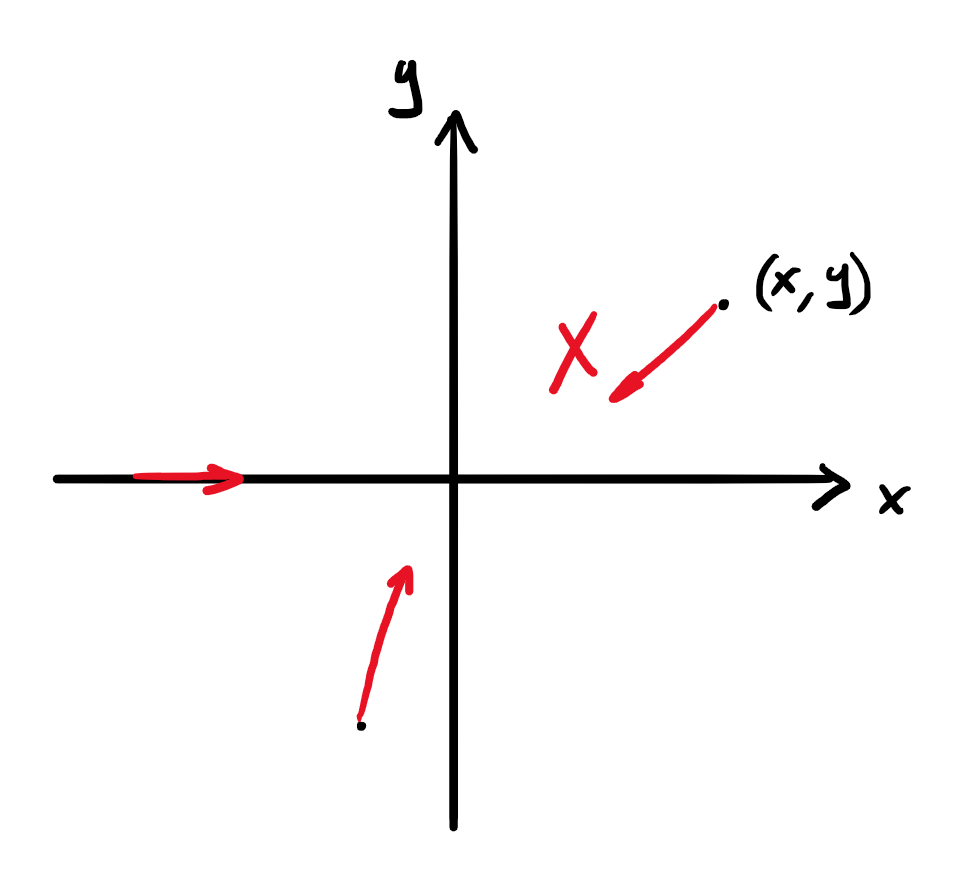
\includegraphics[width=0.4\textwidth,keepaspectratio]{img2}
\end{figure}

Questo campo è liscio perché qualsiasi derivata non annulla mai il denominatore in quanto l'origine non è compresa.

\paragraph{2.}

\begin{align}
	\begin{split}
		X : U = \R^{2} \setminus \{(0,0)\} &\to T_{(x,y)}(\R^{2})\\
		(x,y) &\mapsto X = - \dfrac{y}{\sqrt{x^{2}+y^{2}}} \dfrac{\partial}{\partial x} - \dfrac{x}{\sqrt{x^{2}+y^{2}}} \dfrac{\partial}{\partial y}
	\end{split}
\end{align}

\begin{figure}[H]
	\centering
	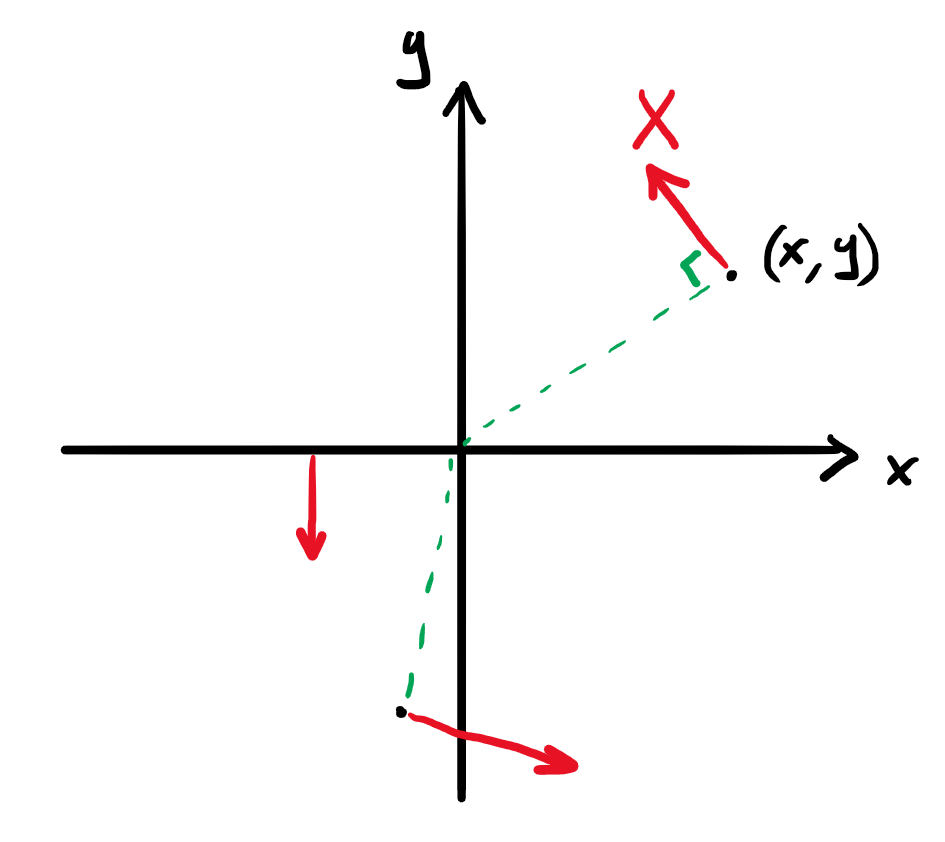
\includegraphics[width=0.4\textwidth,keepaspectratio]{img3}
\end{figure}

Questo campo è liscio perché qualsiasi derivata non annulla mai il denominatore in quanto l'origine non è compresa.

\subsection{Operazioni in $ \chi(U) $}

Si può definire la somma come

\begin{equation}
	(X+Y)_{p} \doteq X_{p} + Y_{p}
\end{equation}

con $ X,Y \in \chi(U) $, questo significa che se

\begin{align}
	\begin{split}
		X &= \sum_{i=1}^{n} a^{i} \, \dfrac{\partial}{\partial x^{i}}\\\\
		Y &= \sum_{i=1}^{n} b^{i} \, \dfrac{\partial}{\partial x^{i}}
	\end{split}
\end{align}

con $ a^{i},b^{i} \in C^{\infty}(U) $, allora

\begin{equation}
	X+Y = \sum_{i=1}^{n} (a^{i}+b^{i}) \, \dfrac{\partial}{\partial x^{i}}
\end{equation}

dove ancora $ a^{i}+b^{i} \in C^{\infty}(U) $ con $ \forall i=1,\dots,n $.\\
Si può definire anche la moltiplicazione per scalari come

\begin{equation}
	(\lambda X)_{p} \doteq \lambda X_{p}
\end{equation}

con $ X \in \chi(U) $ e $ \lambda \in \R $, questo significa che se

\begin{equation}
	X = \sum_{i=1}^{n} a^{i} \, \dfrac{\partial}{\partial x^{i}}
\end{equation}

con $ a^{i} \in C^{\infty}(U) $, allora

\begin{equation}
	\lambda X = \sum_{i=1}^{n} (\lambda a^{i}) \, \dfrac{\partial}{\partial x^{i}}
\end{equation}

dove ancora $ \lambda a^{i} \in C^{\infty}(U) $ con $ \forall i=1,\dots,n $.\\
L'ultima operazione è quella di moltiplicazione di un campo di vettori per un'altra funzione

\begin{equation}
	(f X)_{p} \doteq f(p) X_{p}
\end{equation}

con $ X \in \chi(U) $ e $ f \in C^{\infty}(U) $, questo significa

\begin{equation}
	f X = \sum_{i=1}^{n} (f a^{i}) \, \dfrac{\partial}{\partial x^{i}}
\end{equation}

dove ancora $ f a^{i} \in C^{\infty}(U) $ con $ \forall i=1,\dots,n $.\\
Le prime due operazioni dotano l'insieme di $ \chi(U) $ della proprietà di spazio vettoriale.\\
Osserviamo che $ C^{\infty}(U) $ è un anello commutativo unitario.

\subsection{$ \chi(U) $ come $ C^{\infty}(U) $-modulo}

\subsubsection{$ \R $-modulo sinistro}

Sia $ R $ un anello commutativo unitario, un gruppo abeliano $ (A,+) $ è detto $ R $\textit{-modulo sinistro} se esiste un'applicazione

\begin{align}
	\begin{split}
		\cdot : R \times A &\to A\\
		(r,a) &\mapsto r \cdot a
	\end{split}
\end{align}

tale che

\begin{equation}
	\begin{cases}
		1_{R} \cdot a = a\\
		r \cdot (s \cdot a) = (r s) \cdot a\\
		(r+s) \cdot a = r \cdot a + s \cdot a\\
		r \cdot (a+b) = r \cdot a + r \cdot b
	\end{cases}
\end{equation}

per $ \forall r,s \in R $ e $ \forall a,b \in A $. Queste proprietà valgono solo da \textit{sinistra}, potrebbero non valere se calcolate da destra.

\subsubsection{$ \R $-modulo destro}

Sia $ R $ un anello commutativo unitario, un gruppo abeliano $ (A,+) $ è detto $ R $\textit{-modulo destro} se esiste un'applicazione

\begin{align}
	\begin{split}
		* : A \times R &\to A\\
		(a,r) &\mapsto a * r
	\end{split}
\end{align}

tale che

\begin{equation}
	\begin{cases}
		a * 1_{R} = a\\
		(a*r)*s = a*(r s)\\
		a*(r+s) = a*r + a*s\\
		(a+b)*r = a*r + b*r
	\end{cases}
\end{equation}

per $ \forall r,s \in R $ e $ \forall a,b \in A $. Queste proprietà valgono solo da \textit{destra}, potrebbero non valere se calcolate da sinistra.\\\\
Da queste definizioni, si dice che $ (A,+) $ è un $ R $-modulo se è un $ R $-modulo sinistro e destro, con $ \cdot \equiv * $.

\begin{remark}
	Se un gruppo $ A $ è un $ R $-modulo e $ R $ è un campo $ \K $, allora $ A $ è uno spazio vettoriale in $ \K $.
\end{remark}

\begin{theorem}\label{chi-mod}
	$ (\chi(U),+) $ è un $ C^{\infty}(U) $-modulo.
\end{theorem}

\begin{proof}
	Per dimostrare che $ (\chi(U),+) $ sia un $ C^{\infty}(U) $-modulo, è necessario dimostrare che la seguente applicazione (commutativa)
	
	\map{K}%
		{C^{\infty}(U) \times \chi(U)}{\chi(U)}%
		{(f,X)}{f X}

	sia liscia.\\
	Vedi Esercizio \ref{es1-9}.\\
	Devono dunque essere verificate queste proprietà\footnote{%
		Nonostante l'applicazione sia commutativa, scriveremo la funzione sempre a sinistra dei campi, per notazione.%
	}:

	\begin{equation}
		\begin{cases}
			1_{C^{\infty}(U)} \cdot X = X\\
			f \cdot (g \cdot X) = (f g) \cdot X\\
			f \cdot (X+Y) = f \cdot X + f \cdot Y\\
			(f+g) \cdot X = f \cdot X + g \cdot X
		\end{cases}
	\end{equation}

	per $ \forall f,g \in C^{\infty}(U) $ e $ \forall X,Y \in \chi(U) $.
\end{proof}

\subsection{Derivata di funzione rispetto a un campo di vettori} 

I campi di vettori permettono di derivare funzioni, così come è possibile fare la derivata direzionale di una funzione rispetto a un vettore e dunque rispetto a un campo di vettori.\\
Prendiamo $ X \in \chi(U) $ con $ U \subset \R^{n} $ aperto e $ f \in C^{\infty}(U) $. Definisco la derivata di $ f $ rispetto a $ X $ come $ X f \in C^{\infty}(U) $. La derivata puntuale è definita come $ (X f) (p) = X_{p} f $ con $ p \in U $: se il campo è

\begin{equation}
	X = \sum_{i=1}^{n} a^{i} \dfrac{\partial}{\partial x^{i}}
\end{equation}

allora

\begin{align}
	\begin{split}
		(X f) (p) &= \left( \sum_{i=1}^{n} a^{i}(p) \, \dfrac{\partial}{\partial x^{i}} \right) (f)\\
		&= \sum_{i=1}^{n} a^{i}(p) \, \dfrac{\partial f}{\partial x^{i}} (p)
	\end{split}
\end{align}

perciò

\begin{align}
	\begin{split}
		X f : U \to& \R\\
		p \mapsto& \sum_{i=1}^{n} a^{i}(p) \, \dfrac{\partial f}{\partial x^{i}} (p)
	\end{split}
\end{align}

Questa applicazione è $ C^{\infty}(U) $ perché lo è $ (X f) (p) $, la quale lo è a sua volta perché $ X \in \chi(U) $ in quanto $ a^{i} \in C^{\infty}(U) $ e $ f \in C^{\infty}(U) $.\\
Posso considerare l'applicazione

\begin{align}
	\begin{split}
		X : C^{\infty}(U) &\to C^{\infty}(U)\\
		f &\mapsto X f
	\end{split}
\end{align}

ricordando che $ C^{\infty}(U) $, oltre a essere un anello commutativo unitario, è un'algebra sui reali, perciò l'applicazione $ X $ è $ \R $-lineare. Inoltre, siccome $ X_{p} \in \der_{p}(C_{p}^{\infty}(\R^{n})) $, soddisfa la regola di Leibniz

\begin{align}
	\begin{split}
		X (f g) (p) &= X_{p} (f g)\\
		&= (X_{p} f) \, g(p) + f(p) \, (X_{p} g) 
	\end{split}
\end{align}

perciò anche l'applicazione $ X $ soddisfa la regola di Leibniz

\begin{equation}
	X (f g) = (X f) \, g + f \, (X g)
\end{equation}

\subsubsection{Derivazione di un'algebra}

Sia $ A $ un'algebra\footnote{%
	Un'algebra è costituita da $ (\text{spazio vettoriale},\cdot) $, dove l'operazione
		\begin{align}
			\begin{split}
				\cdot : A \times A &\to A\\
				(a,b) &\mapsto a \cdot b
			\end{split}
		\end{align}
	soddisfa le proprietà
	\begin{equation}
		\begin{cases}
			(a \cdot b) \cdot c = a \cdot (b \cdot c) & \text{associatività}\\
			\begin{split}
				(a + b) \cdot c = a \cdot c + b \cdot c\\
				c \cdot (a + b) = c \cdot a + c \cdot b
			\end{split} & \text{distributività}\\
			\lambda (a \cdot b) = (\lambda a) \cdot b = a \cdot (\lambda b) & \text{omogeneità}
		\end{cases}
	\end{equation}
	per $ \forall a,b,c \in A $ e $ \forall \lambda \in \R $.%
} su un campo $ \K $, un'applicazione $ D : A \to A $ che sia $ \K $-lineare e tale che soddisfi la regola di Leibniz

\begin{equation}
	D (a \cdot b) = (D a) \cdot b + a \cdot (D b)
\end{equation}

per $ \forall a,b \in A $, è chiamata \textit{derivazione dell'algebra} $ A $. L'insieme di tutte le derivazioni di un'algebra $ A $ viene indicato come $ Der(A) $.\\
Vedi Esercizi \ref{es1-10} e \ref{es1-11}.

\subsection{Campo di vettori liscio come derivazione dell'algebra $ C^{\infty}(U) $}

Possiamo vedere un campo di vettori come una derivazione di un'algebra, quindi definiamo un'applicazione

\begin{align}
	\begin{split}
		\phi : \chi(U) &\to Der(C^{\infty}(U))\\
		X &\mapsto \phi(X)
	\end{split}
\end{align}

in cui

\begin{equation}
	\phi(X) (f) \doteq X f
\end{equation}

Sia $ \chi(U) $ che $ Der(C^{\infty}(U)) $ sono $ C^{\infty}(U) $-modulo, dall'applicazione

\begin{align}
	\begin{split}
		K : C^{\infty}(U) \times Der(C^{\infty}(U)) &\to Der(C^{\infty}(U))\\
		(f,D) &\mapsto f D
	\end{split}
\end{align}

da cui

\begin{equation}
	(f D) (g) = f (D g)
\end{equation}

Inoltre $ \phi $ è anche $ C^{\infty}(U) $-lineare, i.e

\begin{equation}
	\phi(f X + g Y) = f \, \phi(X) + g \, \phi(Y)
\end{equation}

per $ \forall f,g \in C^{\infty}(U) $ e $ \forall X,Y \in \chi(U) $.\\
Dimostreremo per le varietà differenziabili che $ \phi $ è un isomorfismo di $ C^{\infty}(U) $-moduli, i.e. $ \chi(U) \simeq Der(C^{\infty}(U)) $.\\
Tramite questo isomorfismo, si possono identificare i campi di vettori lisci con le derivazioni dell'algebra delle funzioni lisce, analogamente a come lo spazio tangente a un punto di $ \R^{n} $ si può identificare con le derivazioni puntuali dell'algebra dei germi delle funzioni in quel punto, i.e. $ T_{p}(\R^{n}) \simeq \der_{p}(C_{p}^{\infty}(\R^{n})) $.